
\begin{frame}[fragile]{Acute Myeloid Leukemia}
\framesubtitle{Definition and diagnosis}

\emph{Acute Myeloid Leukemia} (AML) is one of the most aggressive types of hematological neoplasm, characterized by the infiltration of cancer cells into the \emph{bone marrow}.

\vspace{0.5cm}

\begin{itemize}
\item AML is considered to be a chronic and incapacitating illness;
\item Remission rates \emph{decrease} as the patient ages;
\item The average overall survival rate is only 12 to 18 months \cite{Pelcovits-2020}.
\end{itemize}
\end{frame}



%\begin{frame}[fragile]{Acute Myeloid Leukemia}
%\framesubtitle{Definition and diagnosis}

%\begin{itemize}
%\item For a diagnosis of AML, at least 10\% or 20\% of myeloblasts must be present in the bone marrow or peripheral blood \cite{Arber-2022};

%\item Alongside diagnosis, the patient with AML receives a prognostic of outcomes, divided into three risk categories: \emph{favorable, intermediate, and adverse} \cite{Genomic-2013}; 

%\item  This stratification is defined by cytogenetic and molecular characteristics \cite{Genomic-2013}.

%\end{itemize}
%\end{frame}



\begin{frame}[fragile]{Acute Myeloid Leukemia}
\framesubtitle{Diagnosis and risk stratification}

%The AML risk classification is based on published recommendations made by the European LeukemiaNet (ELN), which became a field of reference in 2010, receiving important updates in 2017 and 2022.  \cite{Dohner-2017} \cite{Dohner-2022}

\begin{center}
    
\begin{figure}
    \centering
    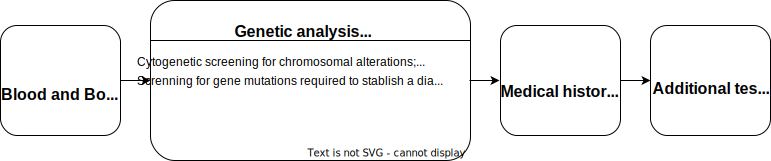
\includegraphics[width=0.9\textwidth]{beamerthemesrc/figs/ELN_classification_pipeline}
    \caption{Simplified diagnosis and risk classification protocol \cite{Dohner-2022}} % <---
    \label{fig:eln_guides}
\end{figure}
\end{center}
    

\end{frame}




\begin{frame}[fragile]{Acute Myeloid Leukemia}
\framesubtitle{Risk stratification and ELN classification}

Specialists commonly use the ELN risk classification to support critical decisions about the course of each treatment, which can directly impact patients' quality of life and life expectancy

\begin{itemize}
\item Patients with a favorable risk prognosis generally present a good response to chemotherapy;

\item Patients with adverse risk exhibit poor response rates to chemotherapy, needing to resort to other treatments, such as stem cell transplantation \cite{Genomic-2013}; 

\item The majority of patients diagnosed with AML are assigned an intermediate-risk classification \cite{Dohner-2010}.

\end{itemize}

\end{frame}



\begin{frame}[fragile]{Acute Myeloid Leukemia}
\framesubtitle{Main concerns about the stratification}

Even though the ELN risk classification is well estabilished in the field, there are main concerns regarding the current risk prognosis:

\vspace{0.25cm}

\begin{itemize}
\item High rate of heterogeneity between patients of the same risk group;

\item No clear definition regarding the intermediate risk since these patients do not show a response pattern to treatments \cite{Dohner-2010}.

\end{itemize}

\vspace{0.25cm}

 To circumvent this problem,  specialists demand more information to support their decisions.
 This process can result in delayed initiation of treatment and consequent worsening of the patient's clinical condition.
 

\end{frame}



%\begin{frame}[fragile]{Decision Support System}
%\framesubtitle{Hypothesis}

%\begin{itemize}
%\item Recent studies show that ML has the potential to generate robust decision support systems to further improve the personalization and recommendation of therapy protocols \cite{Ophir-2019}  \cite{Mosquera-2021} ;

%\item  Experts need to \emph{clearly understand} how the prediction is generated~\cite{Combi-2022};



%\end{itemize}
%\end{frame}





\begin{frame}[fragile]{Decision Support System}
\framesubtitle{Hypothesis}

\begin{block}{In this context...}
This study presents the result of careful analysis of real data composed of clinical and genetic attributes, used to train an \emph{explainable machine learning model} to support therapy protocol decision for AML patients.
\end{block}

With this approach, we aim to: 

\begin{itemize}
    \item Reduce the subjectivity involved in the decision-making process;
    \item Improve time efficiency on selecting the best treatment possible;
    \item Generate robust recommendations with fewer adverse effects, increasing overall survival and quality of life.
\end{itemize}

\end{frame}

